
To show the gaussian variation in the data we collect, figure \refFigure{fig:gauss} depicts a scatter plot of $1000$ sequential runs of the program \bzip, after being compiled using a static inliner (\llvm) whose input was {\tt ebooks}. The figure shows a gaussian noise around the median plus a few outliers, generated by the operating system regular use. These outliers are filtered off from the data we are using. They are easily discarded because they have much more variance (more than one deviation from the median).

\begin{figure}
  \centering
  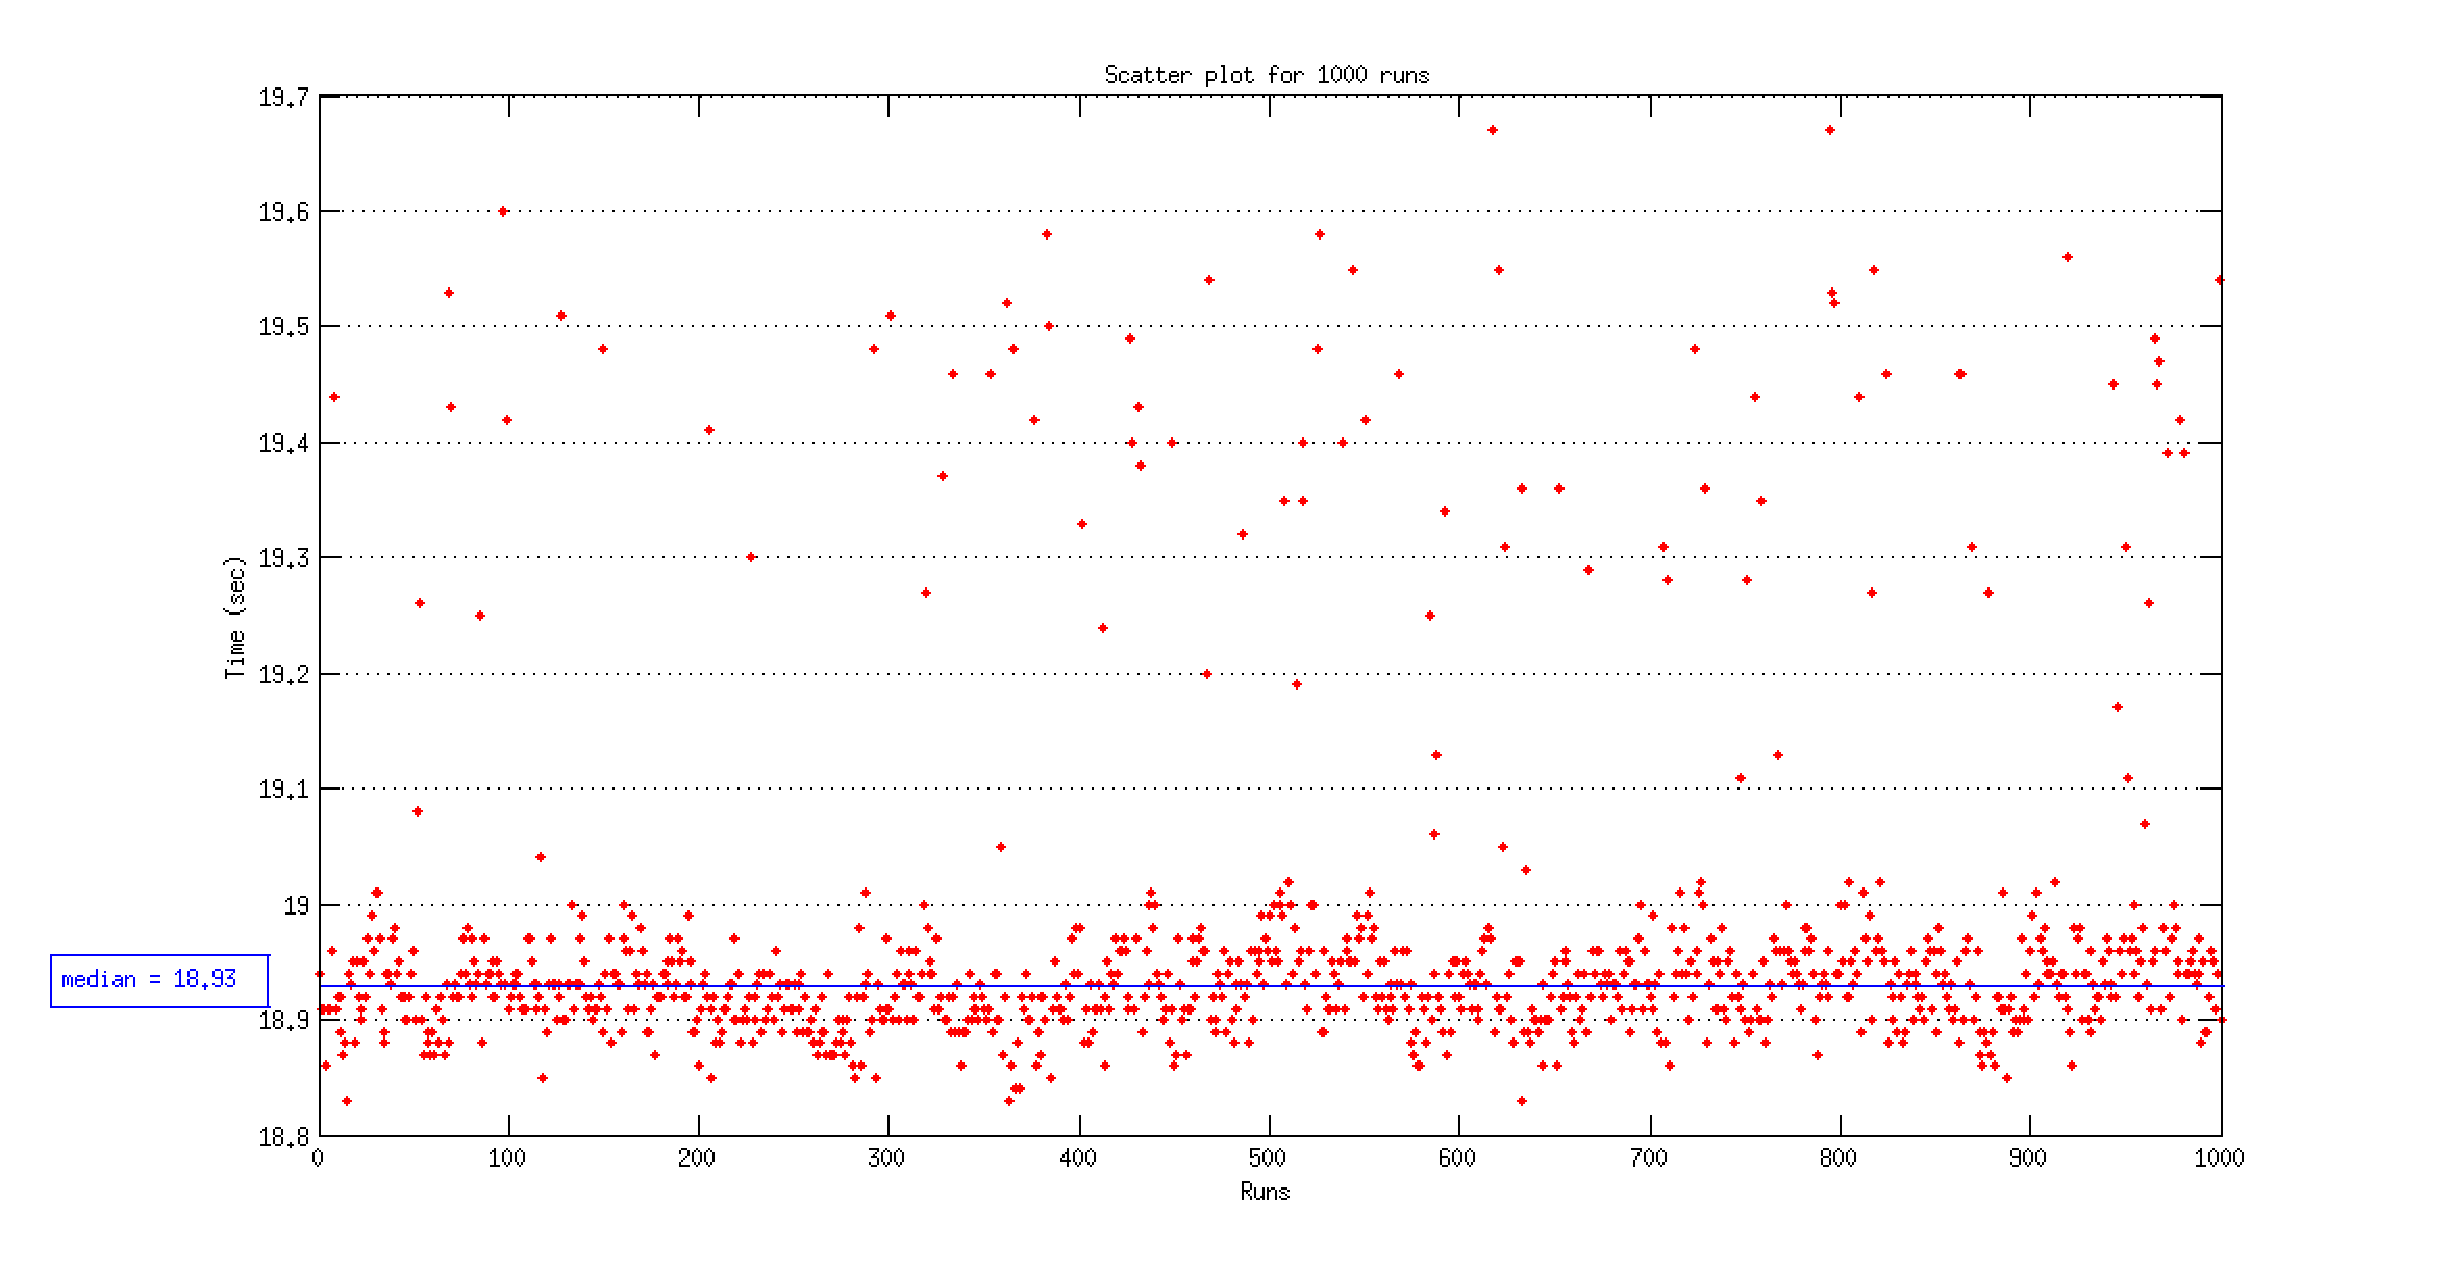
\includegraphics[width=1.00\linewidth]{Figures/1000Runs}
  \caption{Running $1000$ times the same program with the same input data}
  \label{fig:gauss}
\end{figure}

We ran three independent experiments, the first is the $10$-times experiment, then $100$-times and, after that, $1000$-times, because we needed to confirm that there is no difference on their means, and also that we can discard the outliers. To make sure that we have robust measures, we ran some simple statistics to know the mean, the median, the standard-deviation from the mean (std-mean), and the standard-deviation from the median (std-median), shown in \refTable{tab:robustTest}. We also ran t-tests on each sample pairs to verify if their means were the same, the results for the t-tests are shown in \refTable{tab:ttest} below.

\begin{table}
  \centering
  \begin{tiny}
  
\begin{tabular}{lllll}

{\bf Length} & {\bf Mean} & {\bf Median} & 
  {\bf StD Mean} & {\bf StD Median} \\ \hline

10   & 8.7160 & 8.7150 & 0.0100 & 0.0050 \\
100  & 8.7328 & 8.7200 & 0.0187 & 0.0100 \\
1000 & 8.7248 & 8.7200 & 0.0197 & 0.0100 \\

\hline
\end{tabular}

  \end{tiny}
  \caption{Simple statistics on the experiment}
  \label{tab:robustTest}
\end{table}

The t-tests in \refTable{tab:ttest} show that the null hypothesis cannot be discarded, as the value $0$ in each line of the \emph{t-test} column confirms. The \emph{p-values} illustrates the confidence in the hypothesis, in this case, that the means are different.

\begin{table}
  \centering
  \begin{tiny}
  
\begin{tabular}{lllll}

{\bf Runs} & {\bf t-test} & {\bf p-value}  \\ \hline

(10-100) & 0 & 0.3424  \\
(10-1000) & 0 & 0.6025 \\
(100-1000) & 0 & 0.1528 \\

\hline
\end{tabular}

  \end{tiny}
  \caption{t-tests applied pairwise to the $10$, $100$, and $1000$ runs}
  \label{tab:ttest}
\end{table}

\rr{Probably running 3-fold will not be enough, if the running time for a data set is much higher than the running time of this exercise, we have to expect much more noise in the data, but it will be embedded in the data, therefore impossible to extract directly. The only countermeasure is to increase the number of times we run each program from 3 to 5, maybe this could be enough.}

Our experiments have shown that the variance running the same data just three times in a row is not quite different from the $100$ times, when we consider each run a three-fold run, which means running $300$ times the same experiment. What this result means is that we empirically verified the robustness of the \CP\ methodology. As figure \refFigure{fig:CProbust} below shows, the deviation from the mean is not large (\refFigure{CP:mean}), as much as the deviation from the median (\refFigure{CP:median}).  In these figures the $y$-axis reflects the running time for each program on each input data on the $x$-axis.\rr{All other figures in this section figures are dummy}

\begin{figure}
  \centering
  
  \begin{minipage}[t]{\linewidth}
    \subfigure[Each $3$-fold mean run compared with the $300$-times run mean] {
      \begin{minipage}[b]{0.45\textwidth}
        \centering
        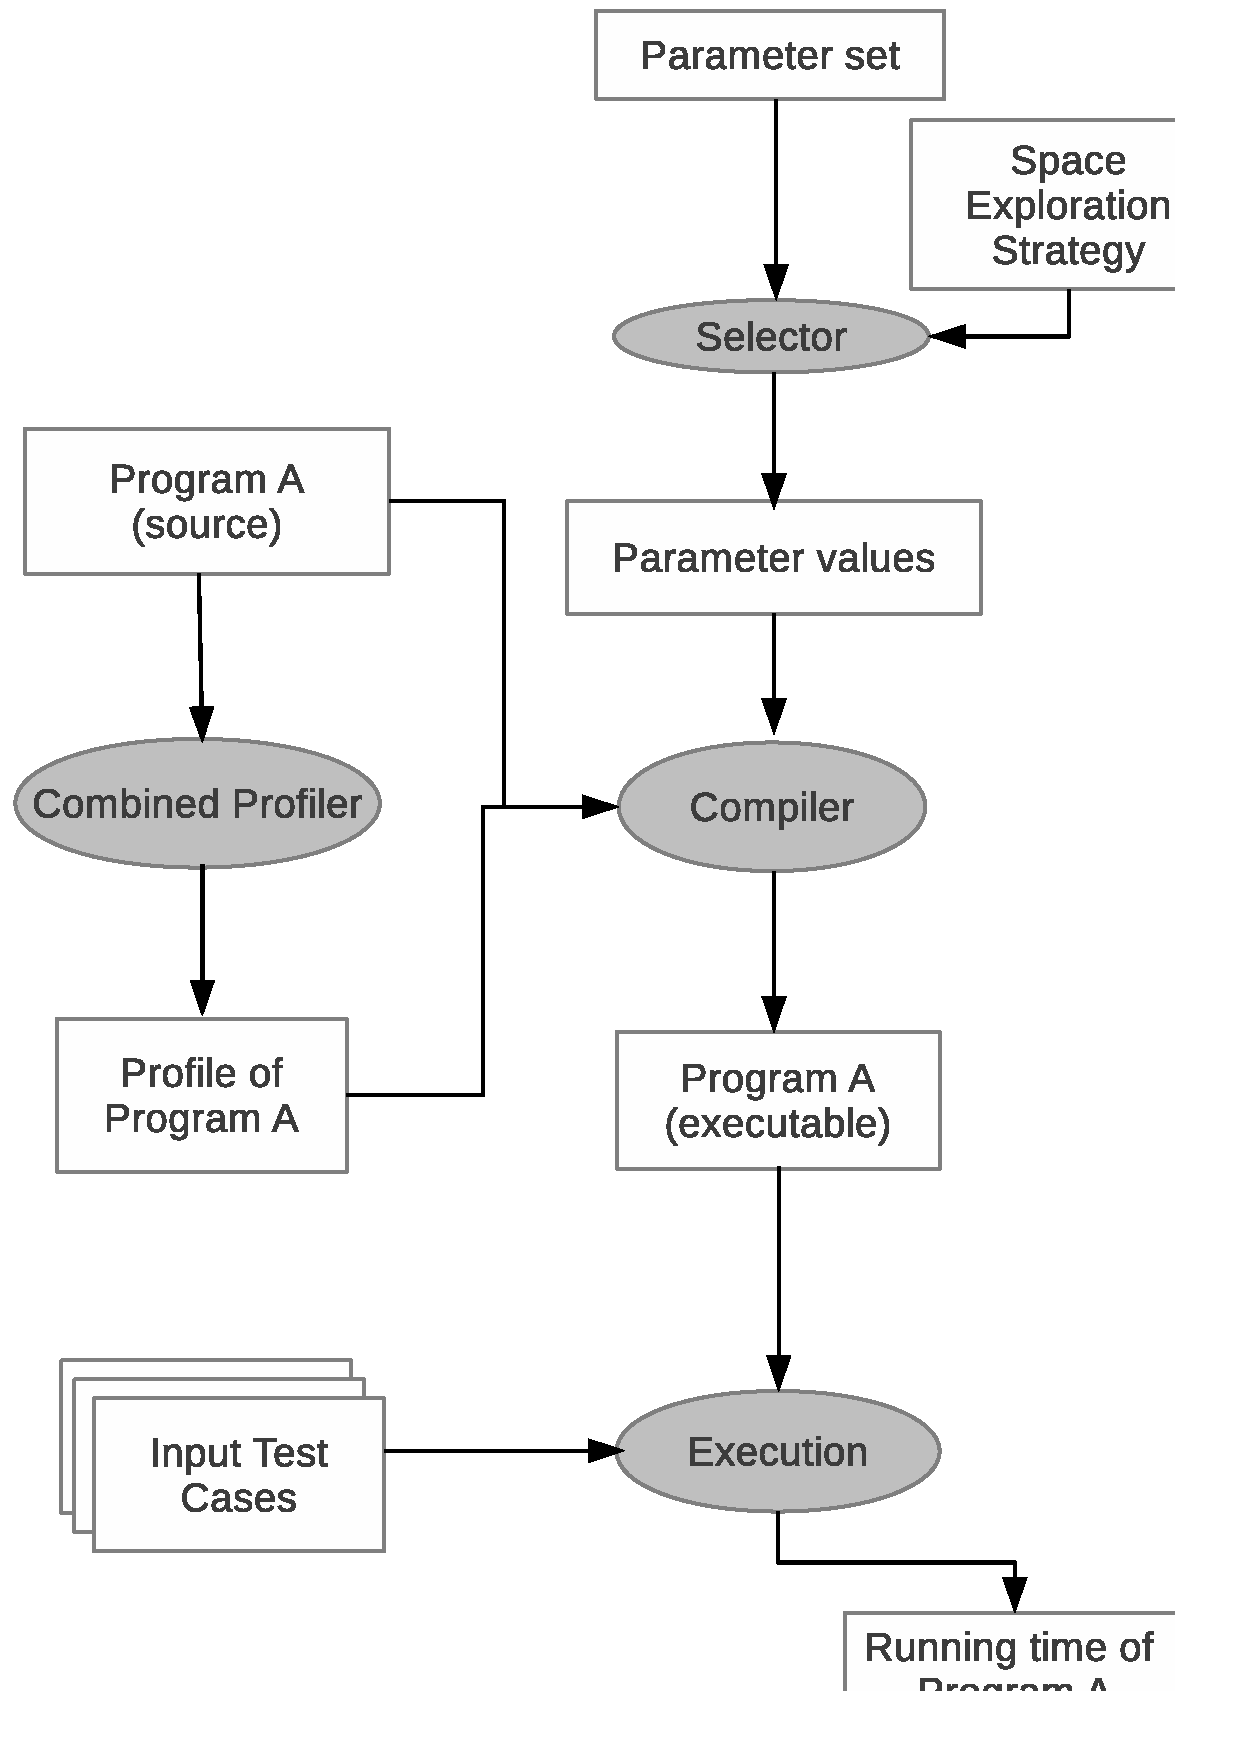
\includegraphics[height=12em]{Figures/CPmean}
      \end{minipage}
      \label{CP:mean}
    }
    \subfigure[Each $3$-fold median run compared with the $300$-times run median] {
      \begin{minipage}[b]{0.45\textwidth}
        \centering
        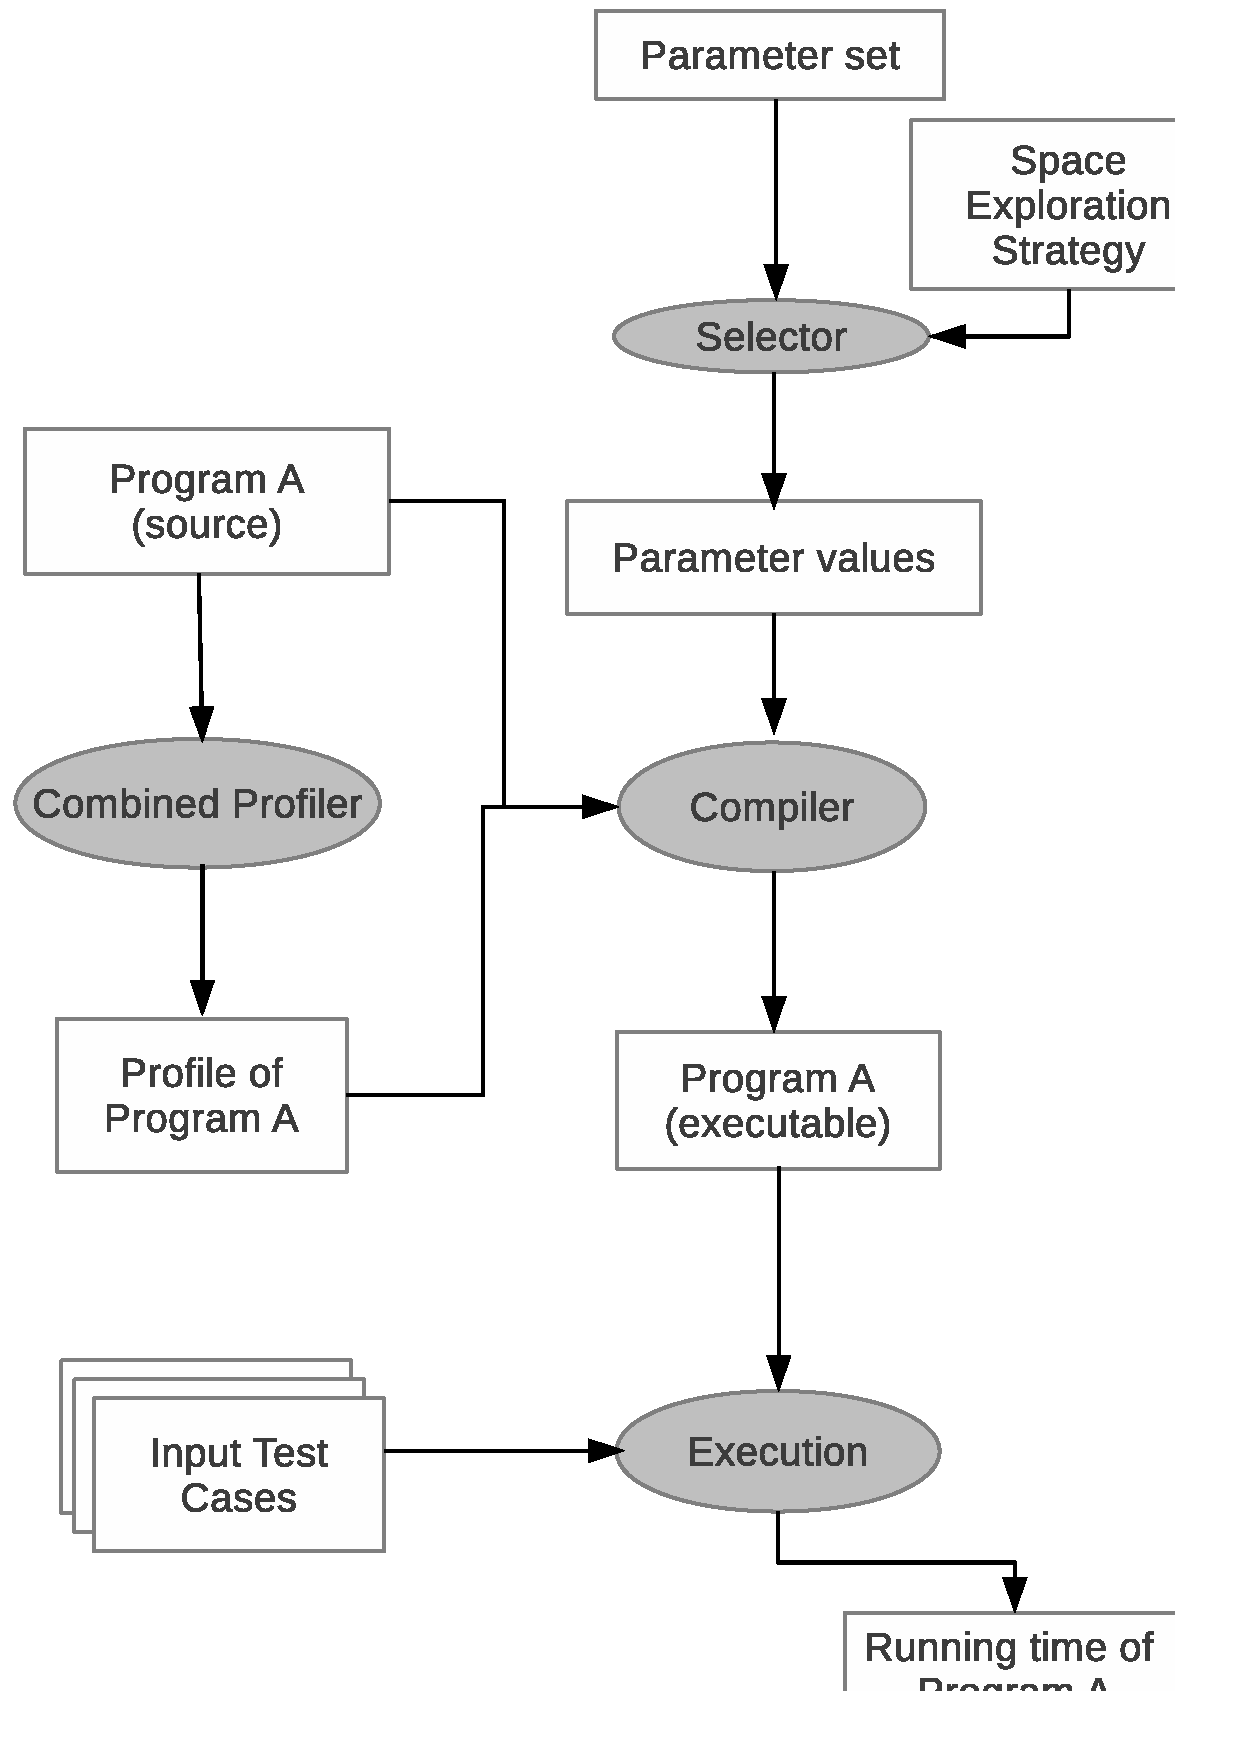
\includegraphics[height=12em]{Figures/CPmedian}
      \end{minipage}
      \label{CP:median}
    }
  \end{minipage}
  \caption{$100$-times running $3$-times experiment}
  \label{fig:CProbust}
\end{figure}

The data used in the experiment are shown in \refTable{tab:simStats}, and the deviations from the mean (and median) to each $3$-fold run are summarized as the average, minimum, and maximum values, all found on the $300$-times experiment.\rr{All other tables in this section figures are dummy}

\begin{table}
  \centering
  \begin{tiny}
  
\begin{tabular}{lllll}

{\bf Run} & {\bf Mean} & {\bf Median} & 
  {\bf StD Mean} & {\bf StD Median} \\ \hline

1 & 8.7233 & 8.72 & 0.0044   \\
2 & 8.71 & 8.71 & 0.0067 & 0.01   \\
3 & 8.72 & 8.73 & 0.02 & 0.01   \\
4 & 8.7067 & 8.7 & 0.0089 & 0.00   \\
5 & 8.71 & 8.71 & 0.0067 & 0.01   \\
6 & 8.7933 & 8.74 & 0.0778 & 0.01   \\
7 & 8.73 & 8.73 & 0.0067 & 0.01   \\
8 & 8.7233 & 8.71 & 0.0178 & 0.00   \\
9 & 8.73 & 8.73 & 0.0067 & 0.01   \\
10 & 8.7033 & 8.71 & 0.0089 & 0.00   \\
\\
33 & 8.71 & 8.71 & 0.0067 & 0.01   \\
34 & 8.7267 & 8.73 & 0.0044 & 0.00   \\
35 & 8.71 & 8.7 & 0.0133 & 0.00   \\
36 & 8.81 & 8.73 & 0.1133 & 0.01   \\
37 & 8.72 & 8.72 & 0.0133 & 0.02   \\
\\
70 & 8.72 & 8.71 & 0.0133 & 0.00   \\
71 & 8.7133 & 8.72 & 0.0089 & 0.00   \\
72 & 8.7233 & 8.72 & 0.0044 & 0.00   \\
73 & 8.7233 & 8.72 & 0.0044 & 0.00   \\
74 & 8.743333 & 8.74 & 0.0111 & 0.01   \\
75 & 8.7667 & 8.76 & 0.0156 & 0.01   \\
76 & 8.7967 & 8.8 & 0.0111 & 0.01   \\
77 & 8.8133 & 8.82 & 0.0089 & 0.00   \\
78 & 8.83 & 8.83 & 0.0067 & 0.01   \\
79 & 8.8433 & 8.84 & 0.0111 & 0.01   \\
80 & 8.74 & 8.74 & 0 & 0.00   \\
81 & 8.7833 & 8.78 & 0.0111 & 0.01   \\
82 & 8.77 & 8.77 & 0.0067 & 0.01   \\
83 & 8.7667 & 8.76 & 0.0222 & 0.02   \\
84 & 8.79 & 8.79 & 0.0067 & 0.01   \\
85 & 8.7633 & 8.76 & 0.0044 & 0   \\
86 & 8.7533 & 8.76 & 0.0156 & 0.01   \\
87 & 8.7467 & 8.74 & 0.0089 & 0.00   \\
88 & 8.74 & 8.74 & 0.0067 & 0.01   \\
89 & 8.7567 & 8.76 & 0.0111 & 0.01   \\
90 & 8.7267 & 8.72 & 0.0156 & 0.01   \\
91 & 8.71 & 8.71 & 0.0067 & 0.01   \\
\\
92 & 8.7133 & 8.71 & 0.0044 & 0   \\
93 & 8.79 & 8.75 & 0.0733 & 0.03   \\
94 & 8.7167 & 8.72 & 0.0044 & 0   \\
95 & 8.72 & 8.71 & 0.0133 & 0   \\
96 & 8.73 & 8.73 & 0.00 & 0.00   \\
97 & 8.73 & 8.74 & 0.02 & 0.01   \\
98 & 8.73 & 8.74 & 0.02 & 0.01   \\
99 & 8.7133 & 8.72 & 0.0089 & 0   \\
100 & 8.7367 & 8.74 & 0.0178 & 0.02   \\

\hline
\end{tabular}

  \end{tiny}
  \caption{Deviation from the mean and from the median in the experiment}
  \label{tab:simStats}
\end{table}

We also ran the t-tests to show that the means (and the medians) are statistically representing the same distribution. This is summarized in \refTable{tab:statTest} below.

\begin{table}
  \centering
  \begin{tiny}
  
\begin{tabular}{lllll}

{\bf T} & {\bf C} & {\bf Quantiles (\%)} & 
  {\bf Description} & {\bf Evaluation Name} \\ \hline

P & -- & 25 & first quartile   & QPointQ=25 \\
P & -- & 50 & estimated median & QPointQ=50 \\
P & -- & 75 & third quartile   & QPointQ=75 \\

P & L & 50, 75 & average and optimistic      & QPLinearQ=50,75 \\
P & NL   & 50, 75 &                             & QPSqrtQ=50,75   \\
P & L & 5, 95  & worst and best w/o outliers & QPLinearQ=5,95  \\
P & NL   & 5, 95  &                             & QPSqrtQ=5,95    \\

R & -- & \pair{50}{100} & top half: optimistic & QRangeQ=50,100 \\
R & -- & \pair{25}{75}  & ``central'' average  & QRangeQ=25,75  \\
R & -- & \pair{5}{95}   & average w/o outliers & QRangeQ=5,95   \\

R & L & \pair{0}{25}, \pair{75}{100} & pessimistic and optimistic
  & QRLinearQ=0,25,75,100 \\
R & NL   & \pair{0}{25}, \pair{75}{100} & 
  & QRSqrtQ=0,25,75,100 \\

\hline
\end{tabular}

  \end{tiny}
  \caption{Test on the means and medians}
  \label{tab:statTest}
\end{table}

This experiment brought us confidence in the machine learning method we devised to tune-in the compiler parameters. We considered the possibility of increasing the number of times each individual run need to be performed, in order to achieve low variance in the data; hence we could trust the results. As this experiment has shown, the $3$-fold run is a good choice, because it does not penalize much the total running time. We show these data in \refTable{tab:runTime}.

\begin{table}
  \centering
  \begin{tiny}
  
\begin{tabular}{lllll}

{\bf T} & {\bf C} & {\bf Quantiles (\%)} & 
  {\bf Description} & {\bf Evaluation Name} \\ \hline

P & -- & 25 & first quartile   & QPointQ=25 \\
P & -- & 50 & estimated median & QPointQ=50 \\
P & -- & 75 & third quartile   & QPointQ=75 \\

P & L & 50, 75 & average and optimistic      & QPLinearQ=50,75 \\
P & NL   & 50, 75 &                             & QPSqrtQ=50,75   \\
P & L & 5, 95  & worst and best w/o outliers & QPLinearQ=5,95  \\
P & NL   & 5, 95  &                             & QPSqrtQ=5,95    \\

R & -- & \pair{50}{100} & top half: optimistic & QRangeQ=50,100 \\
R & -- & \pair{25}{75}  & ``central'' average  & QRangeQ=25,75  \\
R & -- & \pair{5}{95}   & average w/o outliers & QRangeQ=5,95   \\

R & L & \pair{0}{25}, \pair{75}{100} & pessimistic and optimistic
  & QRLinearQ=0,25,75,100 \\
R & NL   & \pair{0}{25}, \pair{75}{100} & 
  & QRSqrtQ=0,25,75,100 \\

\hline
\end{tabular}

  \end{tiny}
  \caption{Running time of experiments, considering $3$-times run}
  \label{tab:runTime}
\end{table}

If we had to run more than three times, say $n$ times, the total running time would be increased for a factor of $k$, where $k = \frac{n}{3}$, which, in case $n = 9$, would result in three times the total running time we had in this experiment.
